\documentclass[12pt]{report}
 
\usepackage[utf8]{inputenc}
\usepackage[T1]{fontenc}
\usepackage[german]{babel}
\usepackage{graphicx}
\usepackage{wrapfig}
\usepackage{amsmath}
\usepackage{cleveref}
\usepackage{amsfonts}
\usepackage{amssymb}
\usepackage{tikz}
\usepackage{nicefrac}
\usepackage{mathtools}
\usepackage{cancel}
\usepackage[margin=1in]{geometry}
\usepackage[section]{placeins}

\newcommand{\kq}{\frac{1}{4 \pi \epsilon_0}}
\newcommand{\vabla}{\vec{\nabla}}
\newcommand{\vepsilon}{\varepsilon}
\newcommand{\vphi}{\varphi}
\newcommand{\dd}{\mathrm{d}}
\newcommand{\diff}{\mathrm{d}}
\newcommand{\exam}{\begin{center}
\textbf{Common exam question}
\end{center}}


\newenvironment{solution}{\begin{proof}[Solution]}{\end{proof}}
 
\begin{document}
 
\title{Experimental Physik III}
\author{Andréz Gockel\\Patrick Munnich\\Daniil Akthonka}
 
\date{\today}
\maketitle

\chapter{Aufgaben}

\section{}

\section{}

\section{}

\subsection{}
Newton mechanics LUL

\subsection{}
\[p=\frac{E}{c}\]

\subsection{}
???

\subsection{}
triggereddaniil.jpeg

\subsection{}
Harmonic oscillator solution:
\[x(t)=\frac{F_0}{\omega^2-i\gamma\omega+\omega_0^2}e^{-i\omega t}\]
\[a+ib\times\frac{a-ib}{a-ib}=\frac{a+b}{a^2+b^2}\]

b) and c) ???

\section{}

\subsection{}
Fermat:
\[n_1\sin\theta_1=n_2\sin\theta_2\]
\[n=\frac{c}{v}\]

\subsection{}
You can unfold boxes.

\subsection{}
\exam
\begin{align*}
\sin\theta&=\mathrm{\frac{opposite}{hypotenuse}}\\
\cos\theta&=\mathrm{\frac{adjacent}{hypotenuse}}=\sin\left(\theta-\frac{2}{\pi}\right)\\
\tan\theta&=\mathrm{\frac{opposite}{adjacent}}
\end{align*}

\subsection{}
???

\subsection{}
\[\sin\theta+\vphi=\sin\theta\sin\vphi-\cos\theta\sin\vphi\]

\section{}

\subsection{}
\[F(\omega)=FT[f(t)]=\frac{1}{\sqrt{2\pi}}\int_{-\infty}^\infty e^{i\omega t}f(t)\dd t\]
\[f(t)=FT^{-1}[F(\omega)]=\frac{1}{\sqrt{2\pi}}\int_{-\infty}^\infty e^{-i\omega t}F(\omega)\dd\omega\]

\subsection{}

\[I_T=I_0\frac{1}{1+f\sin^2\left(\frac{\Delta\vphi}{2}\right)}\]
\[f=\frac{4R}{(1-R)^2}\]
I'd suggest reading through the problem, since context is important here. It's the Fabry-Perot experiment.
\[\frac{\Delta\vphi}{2}=2\pi\frac{d}{\lambda}\sqrt{n^2-\sin^2\alpha}\]

\subsection{}
???

\section{}

\section{}

\section{}

\subsection{}
''Literally nothing''

\subsection{}
Homo Ansatz: \[x=A\sin\omega t\]

\subsection{}
Spontane Emission: \begin{align*}\dot{n}_1=-A_{1\to0}n_1\\\dot{n}_0=+A_{1\to0}n_1\end{align*}\\
Photon Absorption\begin{align*}\dot{n}_0=-B_{1\to0}\rho(\nu)n_0\\\dot{n}_1=+B_{1\to0}\rho(\nu)n_0\end{align*}\\
Stimulierte Emission\begin{align*}\dot{n}_0=+B_{1\to0}\rho(\nu)n_1\\\dot{n}_1=-B_{1\to0}\rho(\nu)n_1\end{align*}\\
Gleichgewicht $n_1$:
\[A_{1\to0}n_1-B_{0\to1}\rho(\nu)n_0+B_{1\to0}\rho(\nu)n_1=0\]

\section{}

\subsection{}
\[E_\mathrm{kin}=\frac{1}{2}mv^2\]
\[E=qU\]
\[F_\mathrm{El}=qE\]
\[F_\mathrm{M}=qvB\]

\subsection{}
\[\vabla\cdot\vec{E}=\frac{\rho}{\vepsilon_0}\]
\[\int|\vec{E}|\dd x=\Delta U\]
\[\textrm{Gau\ss scher Satz }|\vec{E}|2\pi r=\frac{Q}{\vepsilon_0}\]

\subsection{}
\[|\vec{k}|^2=\frac{\omega^2}{c^2}\]
\[\textrm{Sphere }V=\frac{4}{2}\pi r^3\]

\subsection{} 
\[F_\mathrm{Auftrieb}=-\rho V\vec{g}\]

\section{}

\subsection{}
\[\sum_{x=0}^\infty=\frac{1}{1-x}\]

\subsection{}
''Literally nothing''

\subsection{}
''\cancel{meth} math''

\subsection{}
Homework 9

\chapter{Themen}

\section{Relativitäts Theorie}

\subsection{Experimente}
\paragraph{Fizeau-Experiment}

In den beiden Rohren der Länge l fließt eine Flußigkeit mit dem Brechungsindex $n$ mit einer Geschwindigkeit $v$. Licht der Wellenlänge $\lambda$ wird durch einen Strahlteiler (BS) aufgeteilt, und die beiden Strahlen werden von den Spiegeln M2, M3, M4 so reflektiert, dass sie vor dem Auftreffen auf die Kamera die gleiche Strecke zur"ucklegen; der eine Strahl im Uhrzeigersinn (BS $\to$ M2 $\to$ M3 $\to$ M4 $\to$ BS) und der Andere gegen den Uhrzeigersinn (BS $\to$ M4 $\to$ M3 $\to$ M2 $\to$ BS).

\begin{figure}
\centering
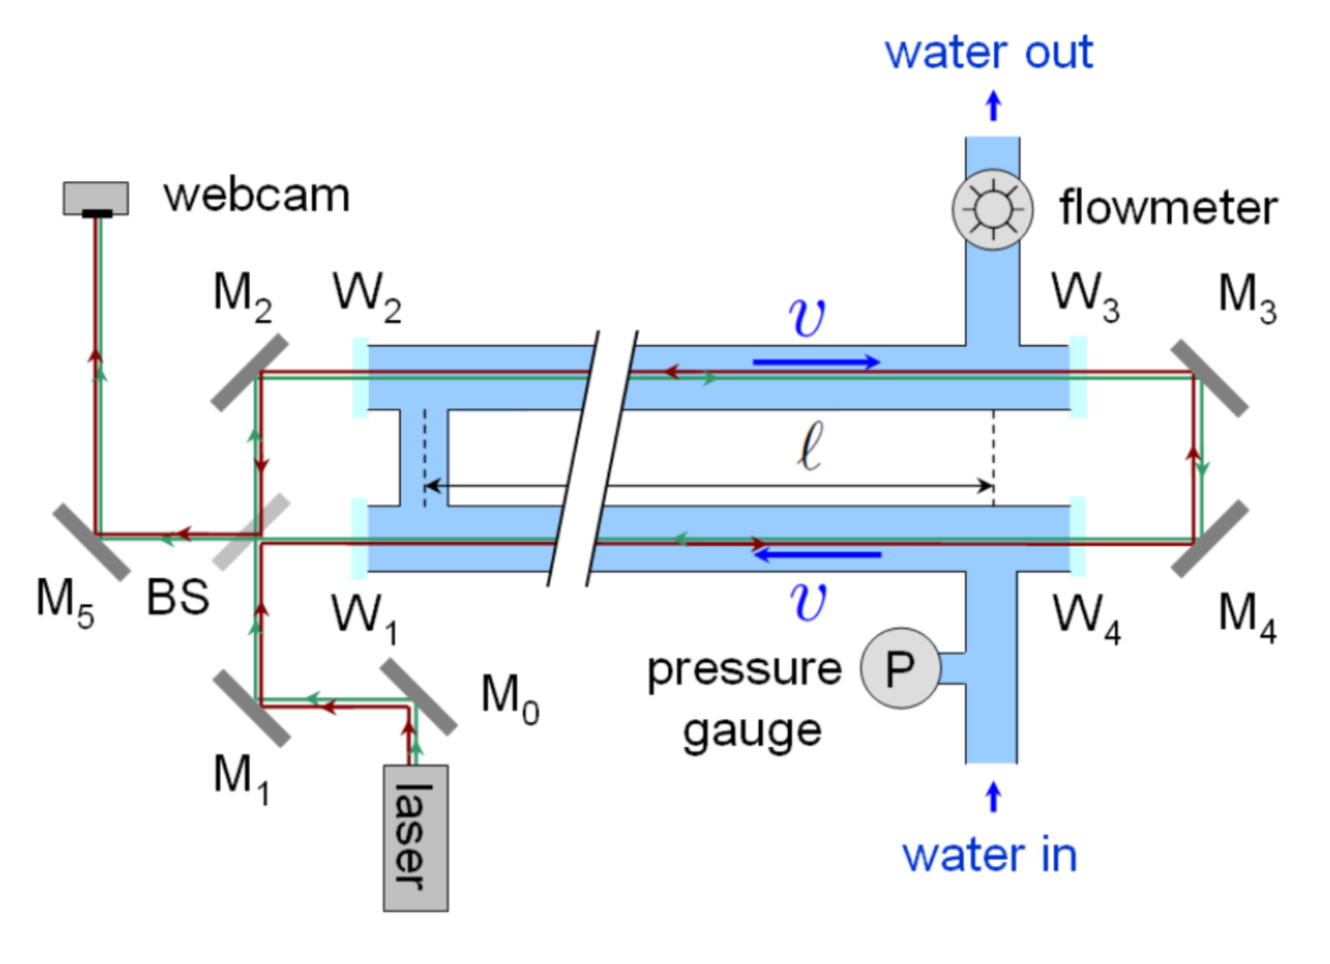
\includegraphics[width=.8\textwidth]{Fizz}
\caption{Fizeau-Experiment}
\label{fizz}
\end{figure}


\chapter{Skript}




\end{document}